\documentclass[onecolumn,10pt,cleanfoot]{asme2ej}

\usepackage{graphicx} %% for loading jpg figures
\usepackage{bm}
\usepackage{nicefrac}
\usepackage{mathtools}
\usepackage{amssymb}
\usepackage{amsmath}
\usepackage{parskip}
\usepackage{listings}
\usepackage{tablefootnote}
\usepackage{float}
\usepackage{xcolor}
\usepackage{xurl}

\definecolor{codegreen}{rgb}{0,0.6,0}
\definecolor{codegray}{rgb}{0.5,0.5,0.5}
\definecolor{codepurple}{rgb}{0.58,0,0.82}
\definecolor{backcolour}{rgb}{0.95,0.95,0.92}

% \expandafter\def\expandafter\UrlBreaks\expandafter{\UrlBreaks%  save the current one
%   \do\a\do\b\do\c\do\d\do\e\do\f\do\g\do\h\do\i\do\j%
%   \do\k\do\l\do\m\do\n\do\o\do\p\do\q\do\r\do\s\do\t%
%   \do\u\do\v\do\w\do\x\do\y\do\z\do\A\do\B\do\C\do\D%
%   \do\E\do\F\do\G\do\H\do\I\do\J\do\K\do\L\do\M\do\N%
%   \do\O\do\P\do\Q\do\R\do\S\do\T\do\U\do\V\do\W\do\X%
%   \do\Y\do\Z}

\lstdefinestyle{mystyle}{
    backgroundcolor=\color{backcolour},
    commentstyle=\color{codegreen},
    keywordstyle=\color{magenta},
    numberstyle=\tiny\color{codegray},
    stringstyle=\color{codepurple},
    basicstyle=\ttfamily\footnotesize,
    breakatwhitespace=false,
    breaklines=true,
    captionpos=b,
    keepspaces=true,
    numbers=left,
    numbersep=5pt,
    showspaces=false,
    showstringspaces=false,
    showtabs=false,
    tabsize=2
}

\lstset{breaklines=true, style=mystyle}
%% The class has several options
%  onecolumn/twocolumn - format for one or two columns per page
%  10pt/11pt/12pt - use 10, 11, or 12 point font
%  oneside/twoside - format for oneside/twosided printing
%  final/draft - format for final/draft copy
%  cleanfoot - take out copyright info in footer leave page number
%  cleanhead - take out the conference banner on the title page
%  titlepage/notitlepage - put in titlepage or leave out titlepage
%  
%% The default is oneside, onecolumn, 10pt, final

\title{Neural networks for solving regression and classification problems}

%%% first author
\author{Jonatan H. Hanssen
    \affiliation{
	Bachelor Student, Robotics and \\
	Intelligent Systems\\ \\[-10pt]
	Department of Informatics\\ \\[-10pt]
	The faculty of Mathematics and \\
	Natural Sciences\\ \\[-10pt]
    Email: jonatahh@ifi.uio.no
    }
}

\author{Eric E. Reber
    \affiliation{
	Bachelor Student, Robotics and \\
	Intelligent Systems\\ \\[-10pt]
	Department of Informatics\\ \\[-10pt]
	The faculty of Mathematics and \\
	Natural Sciences\\ \\[-10pt]
    Email: ericer@ifi.uio.no
    }
}

\author{Gregor Kajda
    \affiliation{
	Bachelor Student, Robotics and \\
	Intelligent Systems\\ \\[-10pt]
	Department of Informatics\\ \\[-10pt]
	The faculty of Mathematics and \\
	Natural Sciences\\ \\[-10pt]
    Email: grzegork@ifi.uio.no
    }
}


\begin{document}


\maketitle



\section{Abstract}

We developed a Feed Forward Neural Network (FFNN) and applied it to many common datasets used for benchmarking machine learning algorithms. Furthermore, we compared our results to those attained by linear and logistic regression. To optimize our network, we explored the use of different schedulers in our gradient descent method, and compared their performance against eachother. Overall, we found that our FFNN performed well in all classification tasks we tested, attaining test accuracies between $95$ and $100$ percent for all classification problems. However, we also found that simple logistic regression performed similarly, with a much lower computational cost. For regression on real terrain data, we found that our neural network slightly outperformed our previous polynomial fit, attaining an MSE of MONKEY, PERCENT percent lower than simple linear regression. In our gradient descent, we found that SCHEDULER performed best, being 1 BILLION percent better than the average of all other methods.

%we found our neural net lacking, not being able to beat our polynomial fit from our previous project, and only attaining an MSE of 1 BILLION, which is 2000 BILLION lower than our best polynomial fit of the Franke Function. 


% \tableofcontents
% \newpage

%%%%%%%%%%%%%%%%%%%%%%%%%%%%%%%%%%%%%%%%%%%%%%%%%%%%%%%%%%%%%%%%%%%%%%

% \begin{nomenclature}
% \entry{A}{You may include nomenclature here.}
% \entry{$\alpha$}{There are two arguments for each entry of the nomemclature environment, the symbol and the definition.}
% \end{nomenclature}
%
% The primary text heading is  boldface and flushed left with the left margin.  The spacing between the  text and the heading is two line spaces.

%%%%%%%%%%%%%%%%%%%%%%%%%%%%%%%%%%%%%%%%%%%%%%%%%%%%%%%%%%%%%%%%%%%%%%
\section{Introduction}
Many problems in machine learning cannot be solved analytically. Thus, we turn to numerical methods, but this change implicitly comes with computationally heavy caveats as they require large matrix calculations over many iterations. Finding a solution becomes a waiting game, finding the many solutions of varying hyperparameters in order to make an informed model selection becomes virtually impossible. The problem of model selection is at the heart machine learning, as optimal model selection allows us to make predictions with the greatest possible accuracy. Finding ways around the liminations of numerical methods becomes a must for proper usage of these powerful machine learning tools.

In this paper we will investigate implantations of the numerical optimization technique of gradient descent by researching stochastic gradient descent, along with constant, adaptive and momentum-enhanced schedulers with the aim of decreasing the computational cost of our calculations. We will study different supervised learning models which utilize gradient descent such as linear regression, logistic regression and a feed forward neural network (FFNN) in order to gain an understanding of model selection across regression, binary- and multi-class classification problems.

First, we will give an explanation of the methods and theory used in this paper, followed up by a presentation and critical discussion of our results. Finally, we will provide a conclusion summarizing the core results and lessons.

% Neural Networks are all the rage these days, everyone wants to have a neural network in their home. Ive even seen people install neural networks in their dogs. \cite{ericjona}

% Neural networks are powerful tools, able to solve many different problems with 

%%%%%%%%%%%%%%%%%%%%%%%%%%%%%%%%%%%%%%%%%%%%%%%%%%%%%%%%%%%%%%%%%%%%%%



\section{Method}

\subsection{Theory}

This sections covers the theoretic background which underlies the methods used in this paper.

\subsubsection{Logistic Regression}

As part of the research conducted in this project, we introduce a new type of regression model, known as Logistic regression. This is a powerful, yet simple algorithm used in machine learning for the purpose of approximating a probability associated with the occurrence of a specific event given measured data. The fundamental idea behind logistic regression is based on the exact approach used in Linear Regression, meaning that we wish to describe a relationship between dependent and explanatory variables in terms of a set of estimated parameters. However, in this case we are not using the weighted sum of our basis functions directly, but feeding them into an activation function. This function, often the sigmoid function, maps the reals onto a range $y \in (0,1)$. This in turn allows for the computation of probability related to an event taking place. Rounding of said probability leads to labeling of each input as belonging to one of two classes, meaning that each object fed into the model will be classified as being of class 0 or 1 (in the case of binary classification).

% To begin with however, the probability output by the activation function will be incorrect for majority of inputs, due to the random nature of the initialized parameters. While this may seem to be an issue, the weights can be adjusted to give better classification results through the application of the gradient descent coupled with an adjustable variable called learning rate. As we also shall see, the implementation of an activation function at the output gives a significant advantage over the classic Linear regression in terms of classification power.
 

\subsubsection{Gradient Descent}

In our previous project, we have primarily dealt with problems that have an analytical solution. This means that once a model has been decided on (polynomial degree and value for lambda for example), finding the optimal solution is a deterministic process which does not require further tuning. However, for the methods we use in this project - such as Logistic Regression - no analytical solutions exist, thus we will have to turn to numerical techniques to find the 'ideal' solution. Our method of choice in this case is gradient descent, an optimization technique which reduces the residuals by utilizing the idea of moving downhill a convex function until a globally minimal scalar value is reached. The gradient itself is nothing more than a first order derivative of a given function, which points in the direction of the greatest change. 

The application of gradient descent to our problems as means of finding the ideal solution implies that the parameters be initialized randomly. The most common approach is to set each parameter equal to a normal distribution with mean zero and variance equal to one, and iteratively update the parameters by calculating the gradient at each given point in the residual space \cite[preface p. x]{dds}. For any one-layer model, the gradient function used to tune the weights will take the form of the product of the partial derivative of the cost function with respect to the activation function, and the partial derivative of the activation function with respect to the weights: 

\begin{equation}
\frac{\partial{\cal C}}{\partial w_{jk}}  = \frac{\partial C}{\partial a_{j}}\frac{\partial a_j}{\partial w_{jk}}
\end{equation}

Although gradient decent is an excellent algorithm for finding optimal solutions, it can also become quite computationally expensive for problems where large numbers of datapoints are available. However, this issue may be effectively countered by applying a variant of standard gradient approach known as Stochastic Gradient Decent or simply SGD. The SGD is based on randomly choosing one or a small number of instances from the dataset to update the parameters, hence the name stochastic. While it may seem like a poor idea to approximate the gradient instead of using the true gradient, the SGD has proven to give a large computational advantage and will often allow the model to converge into a global minima faster than GD. Furthermore, the stochastic nature of this method can allow SGD to avoid getting stuck in local minima \cite[46]{sr}.

\subsubsection{Schedulers}

Whilst SGD itself gives a significant boost to the learning pace of machine learning models, it is possible to improve the algorithm further by performing what is known as scheduling. These methods work by adaptively adjusting the learning rate, thus allowing us to avoid local minima and converge even faster. One of the simpler methods involves adding a fraction of the previous change to the current value used to update the weights, thus keeping a sort of memory of the previous iterations. This is called momentum, due to the physical analogue of a moving particle having momentum. With this addition, we will keep moving in parameter space even if our current gradient is small, because we have gained momentum in a certain direction based on our previous iterations. Furthermore, we will keep moving in the direction where most gradients point, even if outliers point in other directions. Other, more complex methods, also keep track of approximations of the second moment of the cost function. These methods aim to adaptively change the learning rate for different directions in parameter space, so that small steps are taking in steep, narrow directions and large steps taken in shallow, flat directions \cite{mortensched}. Examples of schedulers using the second moment are RMS-prop, Adam and Adagrad.

% Adaptive optimization methods don't always have good generalization. Recent studies have shown that adaptive methods such as ADAM, RMSPorp, and AdaGrad tend to have poor generalization compared to SGD or SGD with momentum, particularly in the high-dimensional limit (i.e. the number of parameters exceeds the number of data points). Although it is not clear at this stage why these methods perform so well in training deep neural networks, simpler procedures like properly-tuned SGD may work as well or better in these applications.

\subsubsection{Feedforward Neural Networks}

For some problems, like approximating a simple function like the Franke Function in project 1, it is sufficient to choose a set of basis functions and find their optimal linear combination. Given that our problem can be reasonably approximated by this basis, we can achieve good results. However, by limiting ourselves to linear functions, we are possibly limiting our model, as our dataset may well be better approximated by a different basis, our perhaps not even by a linear combination of functions at all. Because of this, linear regression is not able to understand the interaction between two arbitrary input variables \cite[165]{gbc}. A better approach would be to simply feed our model our features directly, and hope that it may somehow learn the relationship organically.

To learn any arbitrary relationship between our features may at first seem like an intractable problem, but we are actually able to achieve this with relatively small changes to our linear regression methods. Instead of having our prediction vector be a linear combination of our input vector, we use the linear combinations of the inputs to create an intermediate vector, and apply an activation function to this vector. The resulting values from this function are either passed to the output as a linear combination again, or sent to another intermediate vector. By having the activation function be a nonlinear function, such as the sigmoid or RELU function, we are able to approximate any continous function to arbitrary accuracy \cite[230]{cmb}. By introducing these intermediate vectors, we have created a layered structure, where information is fed forward from layer to layer. Because of this, we call this model a Multilayer Perceptron or a Feedforward Neural Network.

Mathematically, each node on a layer is a linear combination of all the nodes of the previous layer, fed into the activation function for the current layer.

\begin{equation}
a_i^l = f^l(z_i^l) = f^l\left(\sum_{j=1}^{N_{l-1}} w_{ij}^l a_j^{l-1} + b_i^l\right).
\end{equation}

% For an FFNN with an arbitrary amount of hidden layers, the output layer is thus defined as
%
% \begin{equation}
% a^{l+1}_i = f^{l+1}\left[\!\sum_{j=1}^{N_l} w_{ij}^3 f^l\left(\sum_{k=1}^{N_{l-1}}w_{jk}^{l-1}\left(\dots f^1\left(\sum_{n=1}^{N_0} w_{mn}^1 x_n+ b_m^1\right)\dots\right)+b_k^2\right)+b_1^3\right].
% \end{equation}
%
% \begin{equation}
% 	a^{L}_i = f^{L}\left[\!\sum_{j=1}^{N_{L-1}} w_{ij}^3 f^{L-1}\left(\sum_{k=1}^{N_{L-2}}w_{jk}^{L-2}\left(\dots f^1\left(\sum_{n=1}^{N_0} w_{mn}^1 x_n+ b_m^1\right)\dots\right)+b_k^2\right)+b_1^3\right].
% \end{equation}

\subsubsection{Activation functions}

As we have seen, the behaviour of our neural network is defined by the amount of hidden layers and the amount of nodes in each one (our architecture), but also by our choice of activation functions. For the output layer, the activation is usually easily decided based on the problem (identity for regression problems, sigmoid for binary classification, SoftMax for multiclass). For the hidden layers, the choice of activation function is often decided through a process of trial and error, as this is an area without definitive guiding theoretical principles \cite[188]{gbc}. Below are the definitions of some of the most common activation functions.

The sigmoid is defined as follows:

\begin{equation}
y = \frac{1}{1 + exp(x)}
\end{equation}

As we can see from the equation, this function has a range of $y \in (0,1)$, and for high values of x, the rate of change is very small. This saturation is a problem for gradient descent methods, and especially for backpropagation, as the repeated multiplication of very small gradients can lead to weights barely being updated and training slowing down (or even stopping completely). Because of this saturation, the sigmoid is generally not used as an activation function for the hidden layers \cite[191]{gbc}.

Another activation function is the Rectified Linear Unit, and its cousin, the Leaky Rectified Linear Unit:

\begin{equation}
RELU(x) = \left\{\begin{array}{cc} 0 & \; \; if \; \; x < 0, \\  x & \; \; if \; \; x \ge 0.\end{array}\right.
\end{equation}

\begin{equation}
LRELU(x) = \left\{\begin{array}{cc} -\alpha \cdot x & \; \; if \; \; x < 0, \\  x & \; \; if \; \; x \ge 0.\end{array}\right.
\end{equation}

These do not suffer the same saturation problems displayed by the sigmoid function, and as such are often the default choice of activation for the hidden layers \cite[188]{gbc}.

\subsubsection{Backpropagation}

Like logistic regression, the optimal weights for each layer in an FFNN can not be found analytically, and we have to turn to gradient descent. By repeated use of the chain rule, we are able to calculate the gradient for each layer iteratively, using the gradient of the layer after it and starting at the output. This is simply the reverse mode of automatic differentiation, and is computationally preferred compared to forward mode, where we start at the input layer \cite[416]{sr}. The equations for calculating the gradients in an FFNN, which we will not derive here, are as follows \cite{morten}:

First we calculate the so called delta terms for all layers, starting with the output layer:

\begin{equation}
y_i^l = f^l(u_i^l) = f^l\left(\sum_{j=1}^{N_{l-1}} w_{ij}^l y_j^{l-1} + b_i^l\right).
\end{equation}

We use this term in an iterative process, working backwards through the network with the following equation:

\begin{equation}
\delta_j^l = \sum_k \delta_k^{l+1}w_{kj}^{l+1}f'(z_j^l).
\end{equation}

Using these delta terms, we can calculate the gradients for the weights and biases in each layer:

\begin{gather}
w_{jk}^l\leftarrow  = w_{jk}^l- \eta \delta_j^la_k^{l-1} \\
b_j^l \leftarrow b_j^l-\eta \frac{\partial {\cal C}}{\partial b_j^l}=b_j^l-\eta \delta_j^l
\end{gather}

With the theory explained, we can go on to describe how we have applied it to our problem.

\subsection{Implementation}

We implement the FFNN as a class, using NumPy's many matrix functions. In the instantiation of the class, one is able to specify an arbitrary architecture, and choose activation functions for the output and the hidden layer. The cost function can also be specified, and this, along with the choice of output function, allows the network to be used for regression, binary classification and multiclass classification. By specifying no hidden layers in the architecture, the model can be used for linear and logistic regression as well. Because of this, no explicit implementation of linear and logistic regression has been made, which means that almost all relevant code is contained in \texttt{src/FFNN.py} and \texttt{src/Schedulers.py}. When instatiating the model, we set the weights to normal distributions with mean zero and variance one. We set the bias to $0.1$ as recommended in Goodfellow et Al. \cite[189]{gbc}.

The feedforward part is implemented as a simple matrix vector multiplication, followed by an elementwise application of the chosen activation function. For processing batches of inputs, the same multiplication code is used, but this time the input is the design matrix instead of a single row. Each hidden layer will now contain matrices themselves, consisting of a number of rows equivalent to the batch size and a number of columns equal to the number of nodes in this layer.

The backpropagation is implemented by differentiating all the functions declared when the class is instatiated, and following the algorithm laid out in Hjorth-Jensens lectures \cite{morten}. For batch backpropagation, we accumulate the gradient. In practice this means that the gradient for the weights, normally a matrix the same size as the relevant weight matrix, is now one matrix per element in our batch (in practice implemented as a NumPy array of three dimensions). At the end of the batch, we average all the gradients for each weight matrix together and feed this into our scheduling calculation to determine how much our weights should change.

Training a model is implemented as repeated calls to feedforward and backpropagation, once per batch per epoch. During training, one is able to specify which scheduler to use. These are implemented as a series of classes all inheriting from a base class, and are all implemented following Hjorth-Jensens lectures \cite{mortensched}. For finding the optimal parameters, we implement our own gridsearch which finds the lowest error among combinations of lambda, eta, and parameters used for the scheduling.

For verification that our implementation is working correctly, we train on a simple second degree polynomial, and see that our predicted y value is very close to the actual y value\footnote{see \texttt{src/verification.py}}. See Fig.~\ref{verification}.

\begin{figure}[h]
\centerline{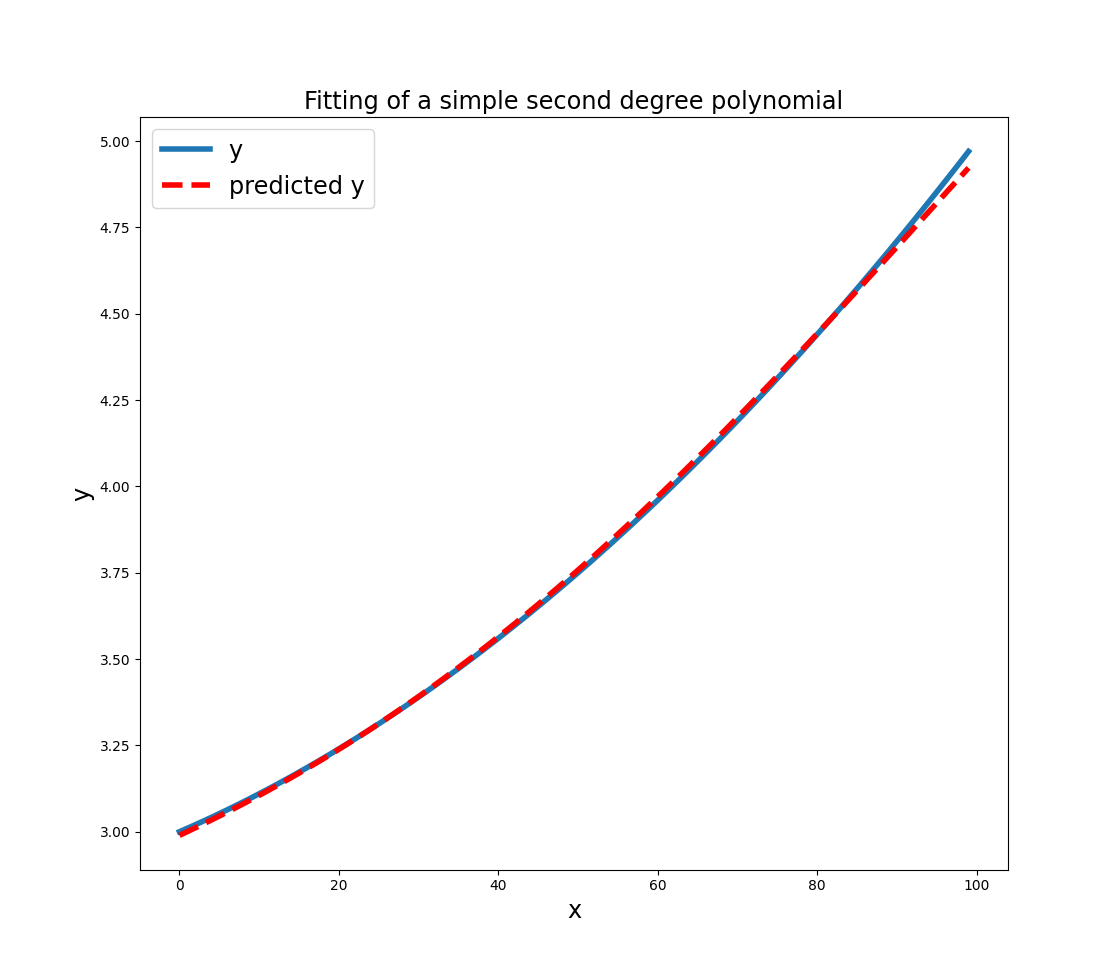
\includegraphics[width=5in]{figure/verification.png}}
\caption{Simple verification case}
\label{verification}
\end{figure}

\subsection{Datasets}

Below is a short description of each dataset used in this report, along with a table (Table.~\ref{datasettable}) listing their characteristics.

\subsubsection{Franke Function}

The Franke Function is a simple weighted sum of polynomials, taking two inputs and returning a real value. It is commonly used to test machine learning algorithms for regression problems.

\subsubsection{Elevation data over Norway}

This data is similar to the Franke Function in that it takes two inputs (x and y coordinates) and returns a real value, which is the elevation of a specific point in Norway.

\subsubsection{Wisconsin Breast Cancer Dataset}

This dataset contains 30 features describing important characteristics of tumors. The features are real numbers. Each instance has an associated class, indicating whether the tumor was benign or not. This leads to a binary classification problem.

\subsubsection{MNIST 8x8}

This dataset contains a preprocessed set of black and white images of hand drawn digits. The images are 8 by 8 pixels, leading to 64 features, where each feature is an integer in the range $[0-16]$ describing the intensity of the pixel at that position\footnote{in reality, this describes the number of "on" pixels in a 4x4 region in the original image}. Each image has an associated class, which is simply the digit depicted. This leads to a multiclass classification problem with 10 classes.

\begin{table}[h]
\caption{Characteristics of each dataset used in the report}
\begin{center}
\label{datasettable}
\begin{tabular}{| c | l | l | l |}
\hline
Dataset & Number of instances & Features & Type \\
\hline
Franke Function & synthetic & 2 & regression \\
Terrain (downscaled) & 204 800 & 2 & regression \\
Wisconsin Breast Cancer & 569 & 30 & binary classification \\
MNIST 8x8 & 1797 & 64 & multiclass classification (10 classes) \\
\hline
\end{tabular}
\end{center}
\end{table}

\section{Results}

\subsection{Different schedulers used with linear regression}

-hessian vs constant?
-constant vs momentum
-adaptive methods
-batch sizes

In order to study the attributes of the different scheduler methods we performed numerical linear regression using gradient descent on the Franke Function. IF HESSIAN: Using Newtons method, the computational cost is much greater than simply replacing the Hessian matrix inversion with a constant learning rate as can be seen by TIME COMPARISON. Furthermore, we can observe from FIGURE COMPARING HESSIAN TO CONSTANT that the constant scheduler does a good job at reducing the MSE, given that the final MSE score is CONSTANTSCORE compared to the Newton method's HESSIANSCORE.

From FIGURE MOMENTUM v CONSTANT we can observe that adding momentum reduces the amount of epochs necessary to reach a lower MSE score. Already after EPOCHS epochs, the momentum scheduler has achieved MOMENTUM MSE AT EPOCHS, a notable improvement over CONSTANT MSE AT EPOCHS achieved by a constant learning rate. Furthermore, with the introduction of various adaptive scheduler methods such as RMS prop, adagrad, adagrad with momentum and adam we can observe from FIGURE ALL that we can reach even greater results in fewer epochs. We can also observe that the different schedulers that they all reach REASONABLE MSE within a couple of epochs, but in order to get a better understanding of the computational cost we have also compared the time it took to fit the data. Looking at TIME TABLE FOR ALL SCHEDULERS, BEST took the least time, beating out our baseline constant scheduler by TIME DIFF. Surprisingly, RMS prop performed more poorly than expected.

Before continuing, it is interesting to note that all the schedulers work best with a combination of similar eta and lambda values when gridsearched for achieving the minimal MSE. It is also interesting that they in the long term reach more or less the same error as can be observed in HEATMAP FIG. This could be because given more epochs, the other schedulers are given more time to catch up as the best performing schedulers, such as Adam, only decrease their MSE slightly. However, as can be seen in HEATMAP FIG, Adam offers a $\frac{0.018}{0.016} \dot 100 = 11.11\%$ decrease in MSE compared to the constant schedulers.

However, when trained for 500 epochs, Adam with optimal parameters does not yield any improvement in MSE. Scikits Adam scheduler does perform better, further decreasing the MSE slightly. Even though we have cross validated both our own Adam implementation and Scikit's with 5 folds, these differences in results might be due to a more favorable weight initiation in Scikits model. Nonetheless, neither models are able to beat the analytical solution provided by linear regression methods using polynomial approximations, with our best result of ADAM FINAL MSE and Scikits final MSE of SCIKIT FINAL MSE both falling short of the analytical MSE of 0,003. In theory, the feed forward neural network should be able to better approximate the Franke function given that it is not limited to polynomial solutions. This result might be due to 500 epochs not being enough training time.

<<<<<<< HEAD
=======
In order to study the attributes of the different scheduler methods we performed a simple linear regression using gradient descent on the Franke Function. IF HESSIAN: Using Newtons method, the computational cost is much greater than simply replacing the Hessian matrix inversion with a constant learning rate as can be seen by TIME COMPARISON. Furthermore, we can observe from FIGURE COMPARING HESSIAN TO CONSTANT that the constant scheduler does a good job at reducing the MSE, given that the final MSE score is CONSTANTSCORE compared to the Newton method's HESSIANSCORE.
>>>>>>> a87b6f80c33cf6ab0163d7ca8f59b55321cd75a0


\subsection{Neural Network for regression}

For the organic terrain data used in our previous project, we found that our neural net performed slightly better, gaining an MSE of NUMBER, which was about PERCENTAGE better than our best polynomial fit. However, looking at our prediction visually, and also comparing the MSE to the one gained on the Franke Function, we see that we are still lacking. For terrain data like this, which contain a lot of spatial information, we believe that Convolutional Neural Networks could be a better fit.

\subsection{Neural Network for binary and multiclass classification}

To test our neural networks ability to solve classification problems, we first applied it to the Wisconsin Breast Cancer dataset. Using our gridsearch method, we found that the best scheduler was Adam, with an eta of $0.01$ and no regularization. For our architecture, we chose to use only one hidden layer with 60 nodes, based on our testing. With this, we were able to achieve a crossvalidated test accuracy of $98.6 \%$, which is very good. Looking at the confusion matrix (Fig.~\ref{cancerconf}), we see that we are achieving good predictions for both true positives and true negatives.

\begin{figure}[h]
\centerline{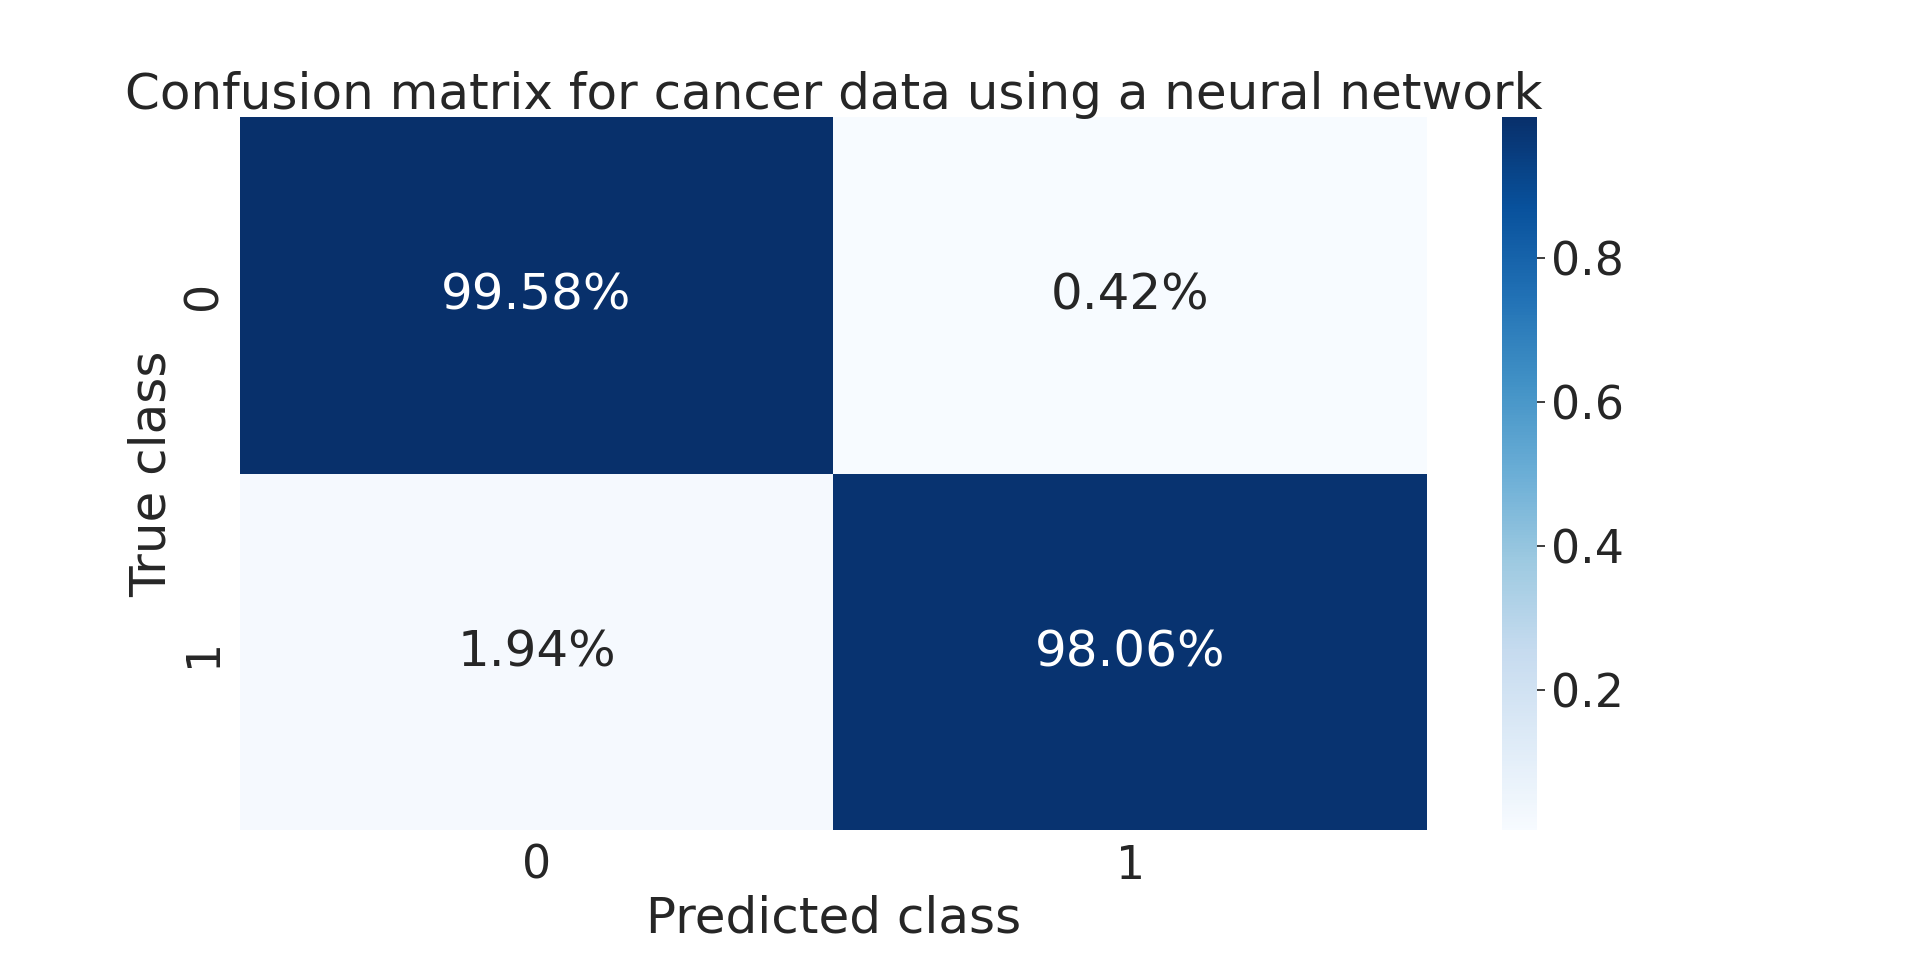
\includegraphics[width=5in]{figure/cancerconf.png}}
\caption{Confusion matrix for the cancer dataset using a neural net with a single hidden layer of 60 nodes}
\label{verification}
\end{figure}

Confident in our networks's ability to to binary classification, we turned to the MNIST dataset. Using our gridsearch, we again found that the best scheduler was Adam. Our architecture in this case was a single hidden layer with 100 nodes. Being a multiclass problem with ten different classes, one might expect our neural network to struggle more with this dataset. However, this was not the case, as we achieved a crossvalidated test accuracy of $99.07$. From these two datasets, we can see that a correctly optimized neural network is adept at solving classification problems. On the other hand, these good results, and the easew with which our network attained them, could imply that the problems we have dealt with are not as complicated as they may seem.

\subsection{Logistic Regression}

Based on our good results with the neural net, we attempt to solve the same problems using simple logistic regression. Using logistic regression on the cancer dataset, we found through our gridsearch that Adam with an eta $0.1$ gave the best results. Here we found that logistic regression performed essentially equivalent or even better, at a much lower computational cost. Looking at Fig.~\ref{cancerlogneur}, we see that logistic regression keeps up and even surpasses our neural network in accuracy per epoch. The value of logistic regression becomes even greater when we consider the computational cost of each method. In this case, the logistic regression was about 65 \% faster\footnote{The time taken to complete a crossvalidation with 5 folds up to 200 epochs was about 52 seconds for our neural network, but only 18 seconds for logistic regression}, with results surpassing our neural network (see Fig.~\ref{cancerconflog}). This implies that our classification datasets were perhaps too simple, and that using Neural Networks was not needed to achieve good results.

\begin{figure}[h]
\centerline{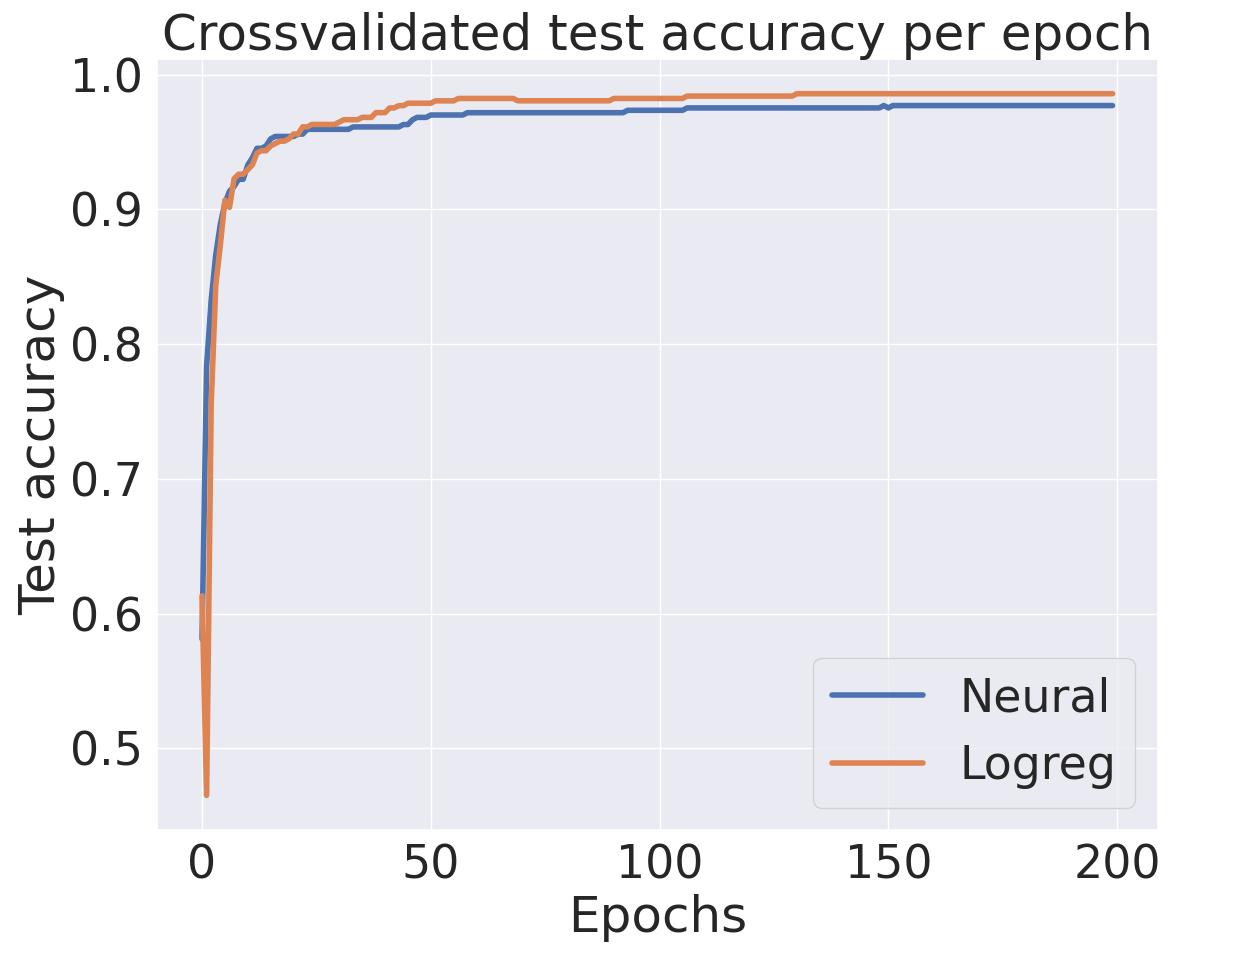
\includegraphics[width=5in]{figure/cancerlogneur.png}}
\caption{Comparison between the test accuracy of logistic regression and a neural network on classifying the cancer dataset}
\label{cancerlogneur}
\end{figure}

\begin{figure}[h]
\centerline{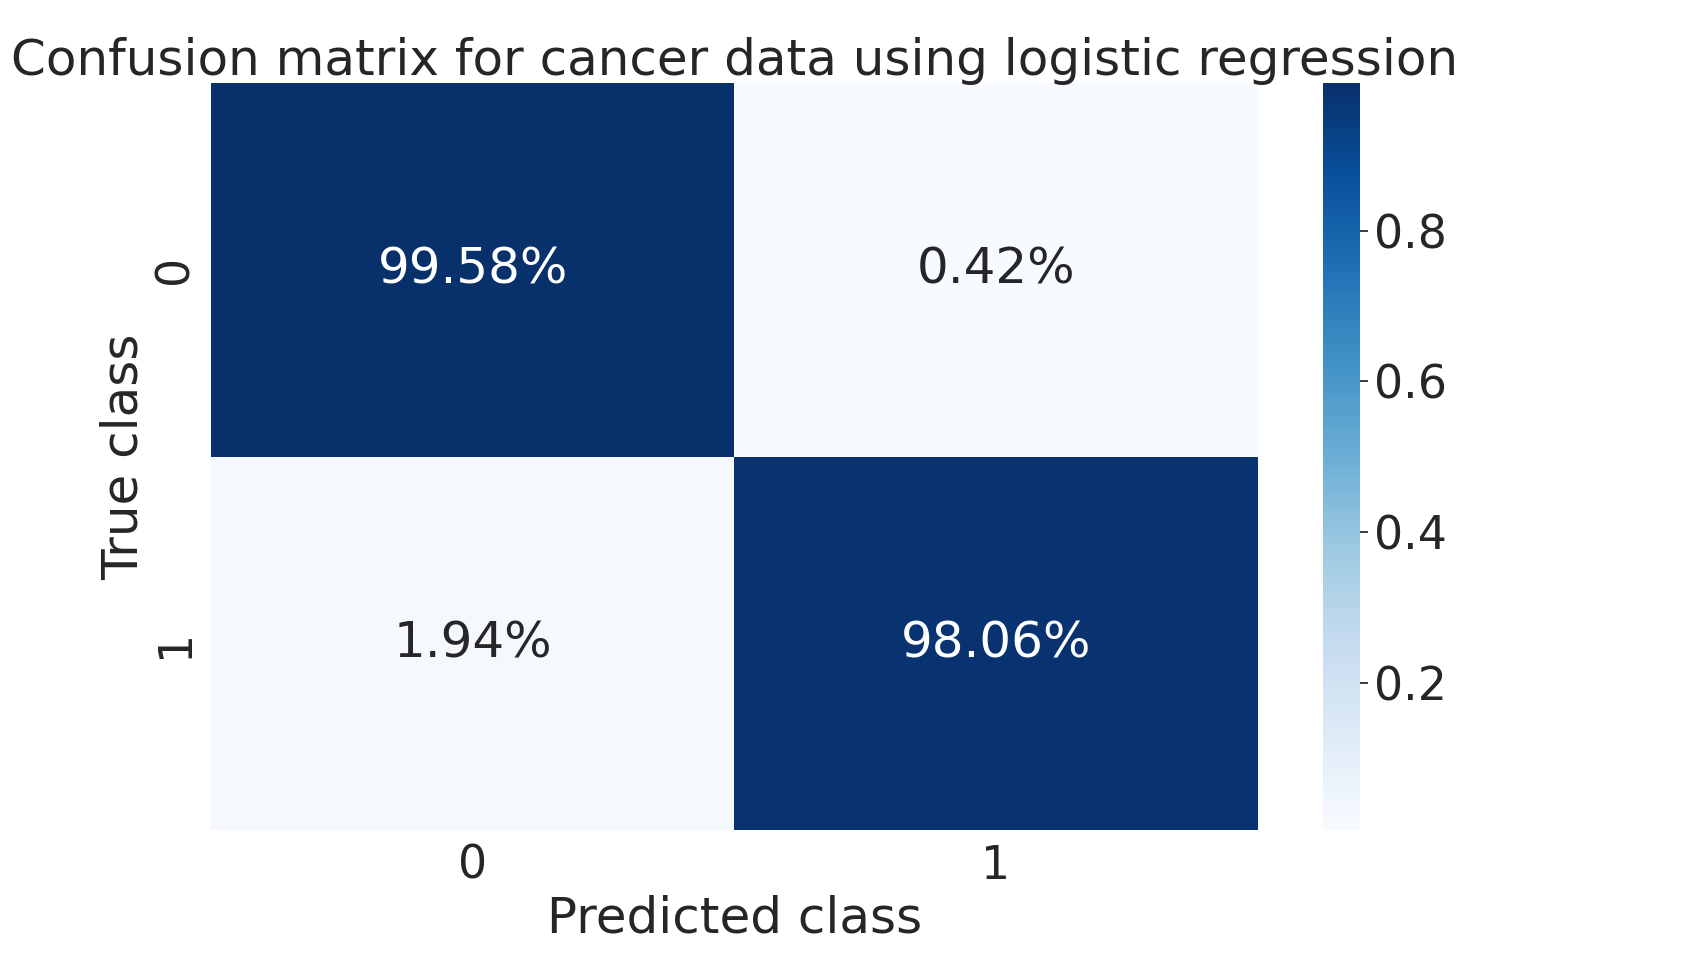
\includegraphics[width=5in]{figure/cancerconflog.png}}
\caption{Confusion matrix for the cancer dataset using logistic regression}
\label{cancerconflog}
\end{figure}

\section{Conclusion}

In this paper we have explored the use of a Feed Forward Neural Network for both regression and classification. We have studied how different schedulers, 

\bibliographystyle{apalike}
\bibliography{bibliography}

\section*{Appendix A: Plots and tables}

The next pages contain plots and tables that are of interest.

\begin{table*}
\caption{This table shows the command to execute to reproduce every figure in the report. (More info about the scripts and their parameters can be found in the README)}
\begin{center}
\label{allparamstable}
\begin{tabular}{c | l l l}
Figure & Shell command (leading \texttt{python3} omitted) \\
\hline
\ref{frankenonoise} & \texttt{task\_b.py --noise 0 -n 25}\\
\hline
\end{tabular}
\end{center}
\end{table*}

\end{document}
